\documentclass[12pt,a4paper,titlepage]{article}

\usepackage{preamble}
\title{Représentation  Temps-Fréquence : travaux pratiques}
\author{Yassine Jamoud, Samy Haffoudhi}
\date{\today}

\begin{document}

\maketitle

\section{Présentation du TP}

Ce TP concerne l'imagerie Synthetic Apperture Focusing Technique (SAFT) pour le
contrôle par ultrasons. Nous nous intéressons au contrôle d'un bloc d'aluminium
contenant des petits trous à l'aide d'une sonde multi-élément en contact direct
avec la pièce. Nous mettrons en œuvre une méthode d'imagerie dite temporelle que
nous commencerons par implémenter dans matlab à l'aide de boucles \texttt{for} avant
de convertir ce code en fonction MEX afin de comparer le temps de calcul des deux
mises en œuvre.

\begin{figure}[H]
    \caption{Principe de l'imagerie SAFT}
    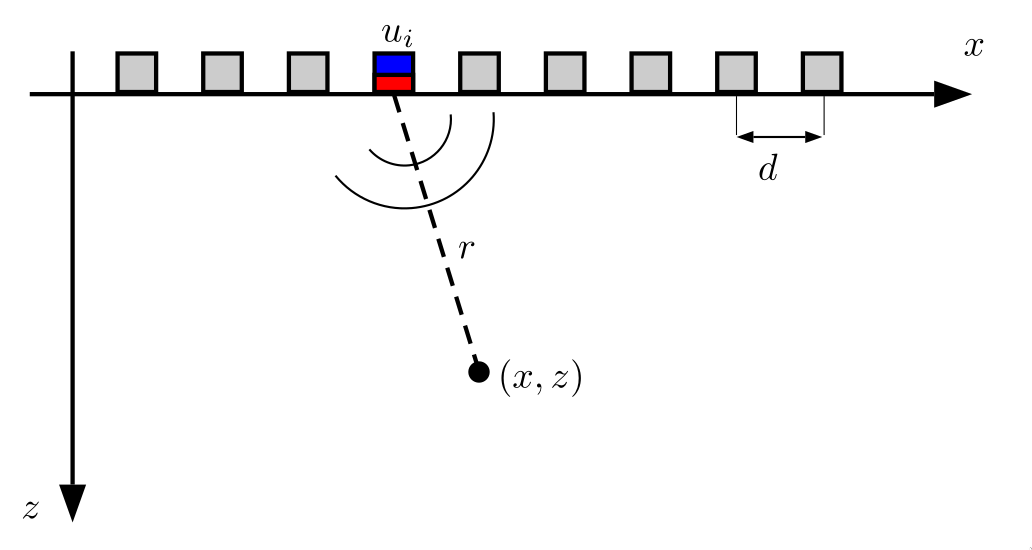
\includegraphics[width=0.6\textwidth]{sujet}
    \centering
\end{figure}

\section{Ouverture du fichier}

\begin{itemize}
    \item{On a $N_t = 1500$ et $N_{el} = 128$.}
    \item{Affichons l'image des données en fonction de $t$ et $u$ :

            \begin{figure}[H]
                \caption{Image des données}
                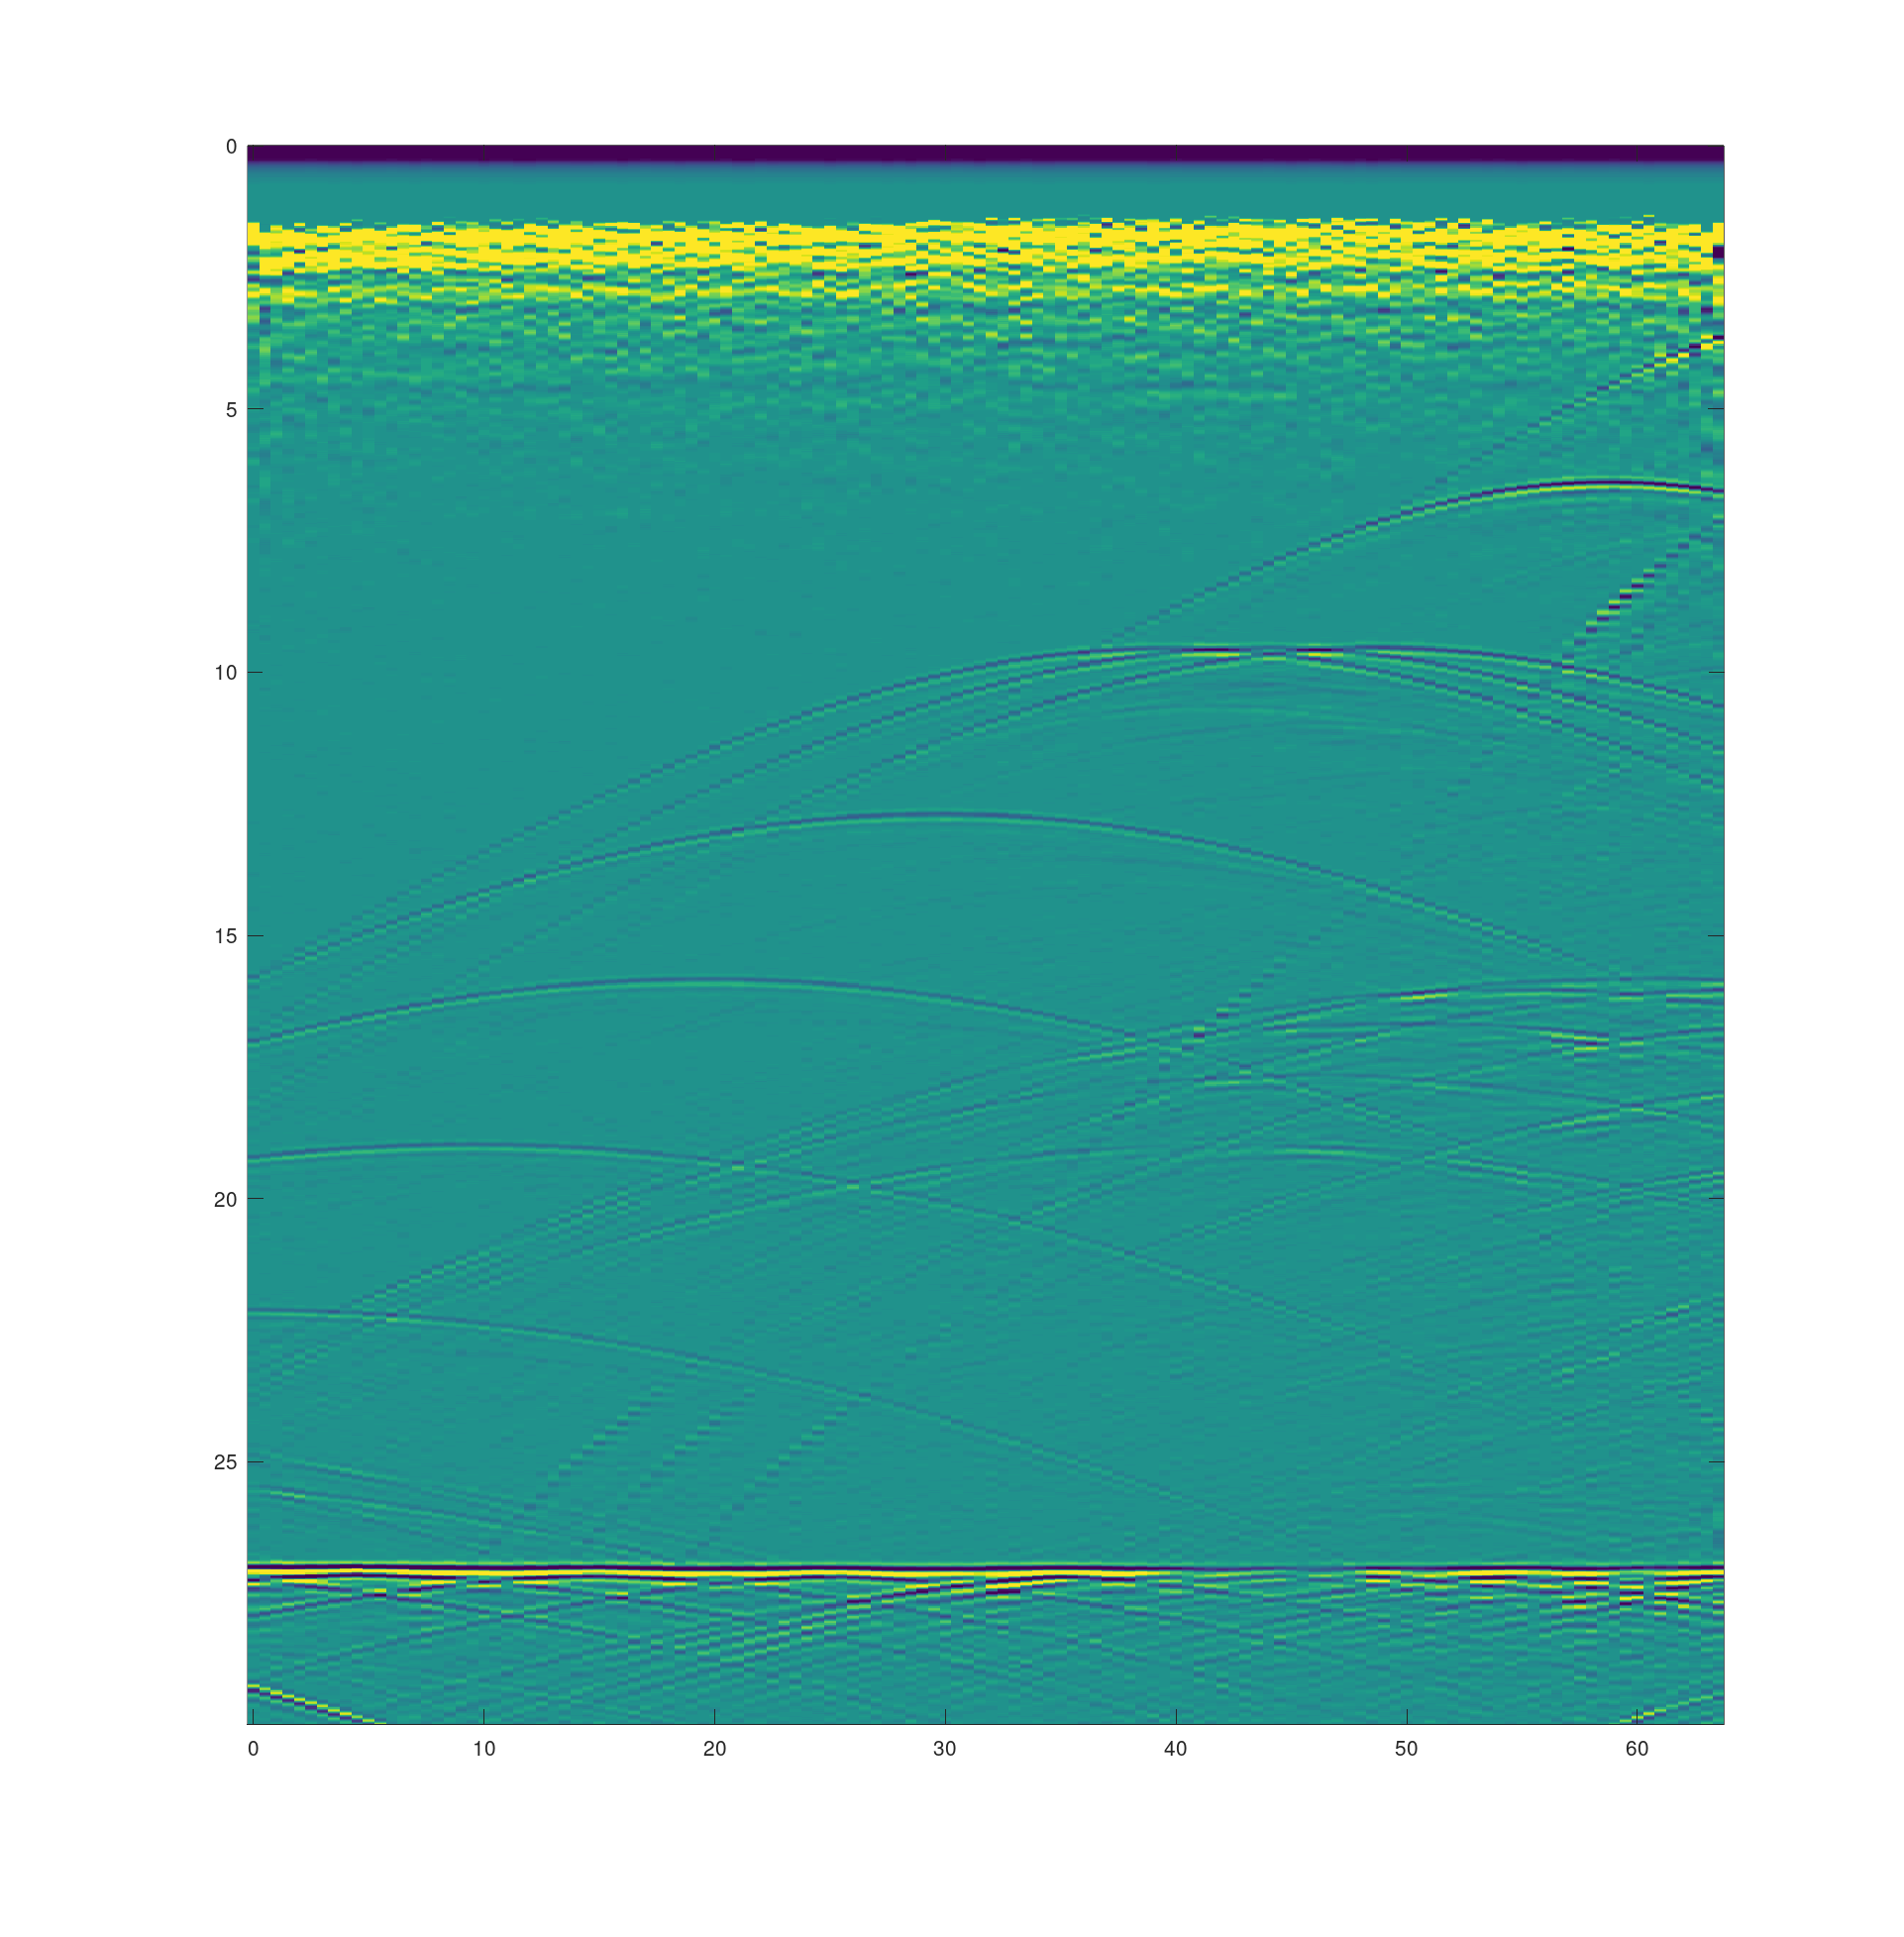
\includegraphics[width=0.5\textwidth]{im1}
                \centering
            \end{figure}
        }
    \item{Cette image n'est pas exploitable, on est incapable d'y distinguer les
        petits trous du bloc d'aluminium.}
    \item{Affichons maintenant un Ascan :

            \begin{figure}[H]
                \caption{Ascan}
                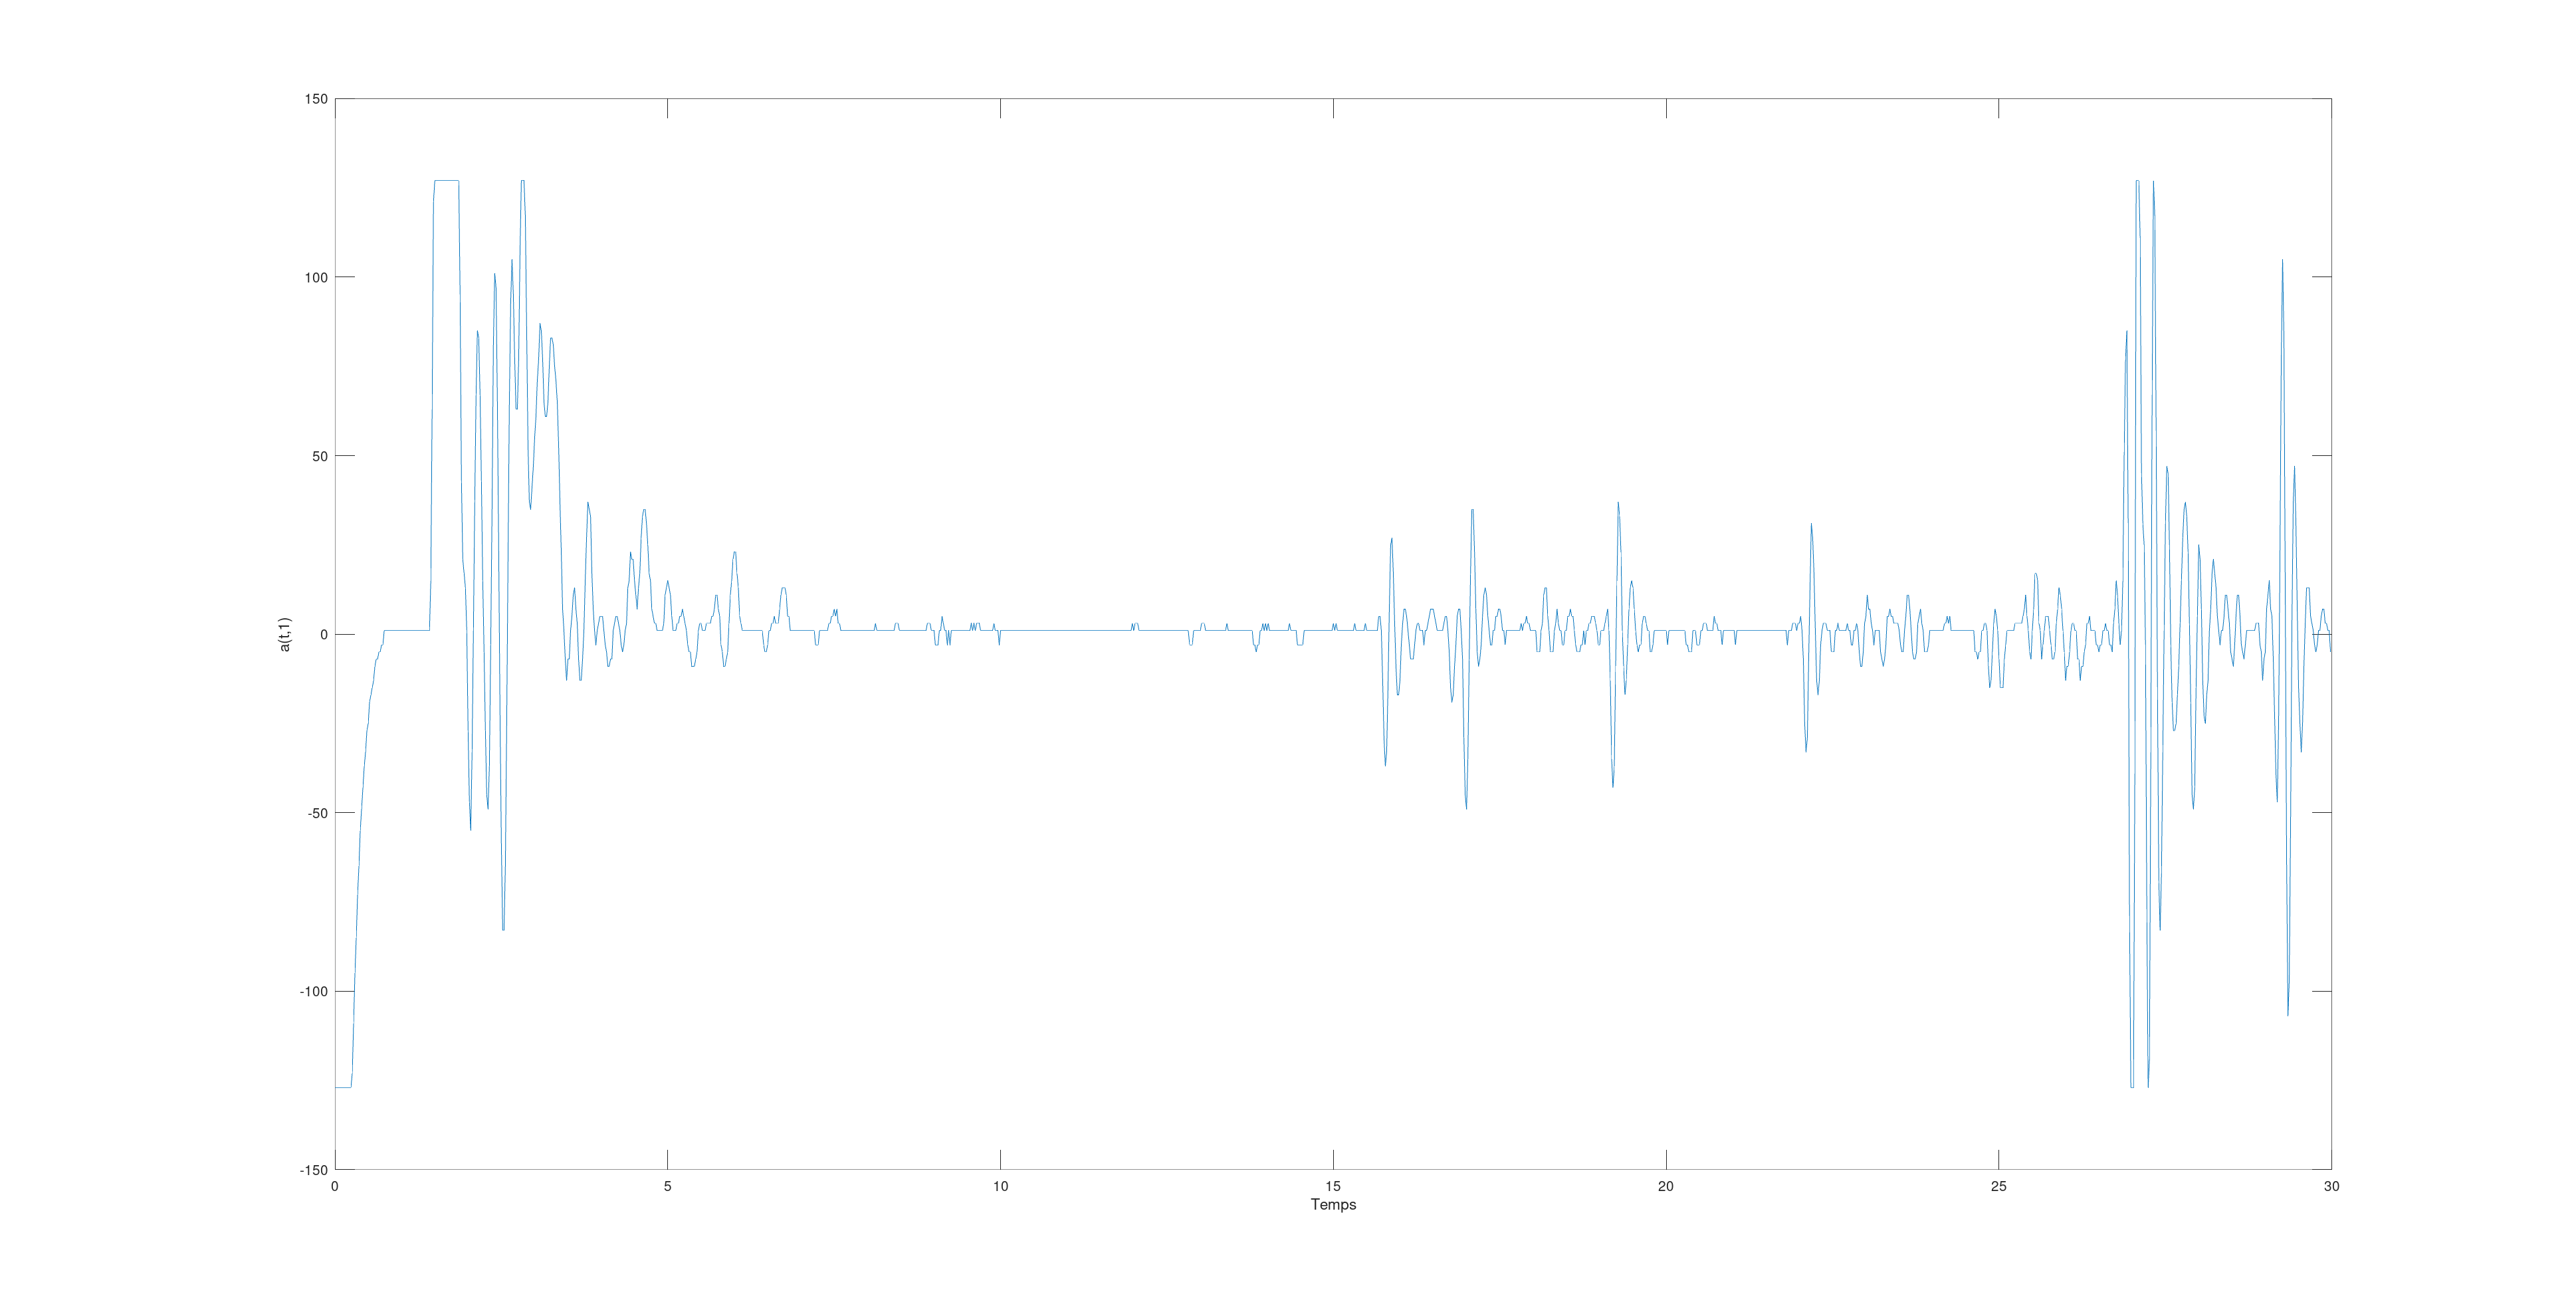
\includegraphics[width=0.7\textwidth]{im2}
                \centering
            \end{figure}
        }
    \item{On déduit de la figure précédente que $log_2(2 \times 128) = 8$ bits sont utilisés.}
\end{itemize}

\section{Définition de la grille de reconstruction}

Nous modifions le fichier \texttt{main.m} disponible en annexe.

\section{Reconstruction de l'image par une méthode temporelle}

\begin{itemize}
    \item{D'après la figure 2, on a : $r(x,z,u_i) = \sqrt{(u_i - x)^2 + z^2}$.}
    \item{On a : $\tau(x, z, u_i) = \frac{2r(x,z,u_i)}{c}$.}
    \item{Donc, on peut calculer $O(x,z) = \sum_{i=1}^{N_{el}}a(\tau(x, z, u_i),i)$.}
    \item{On ajoute la procédure au fichier \texttt{main.m} pour le calcul de $O$.}
    \item{On considère $N_x \in \{64,128,256,512,1024,2048\}$.

            Affichons deux images obtenues :

            \begin{figure}[H]
                \subfloat[$N_x = 64$]{
                    \begin{minipage}[c][1\width]{
                        0.5\textwidth}
                        \centering
                        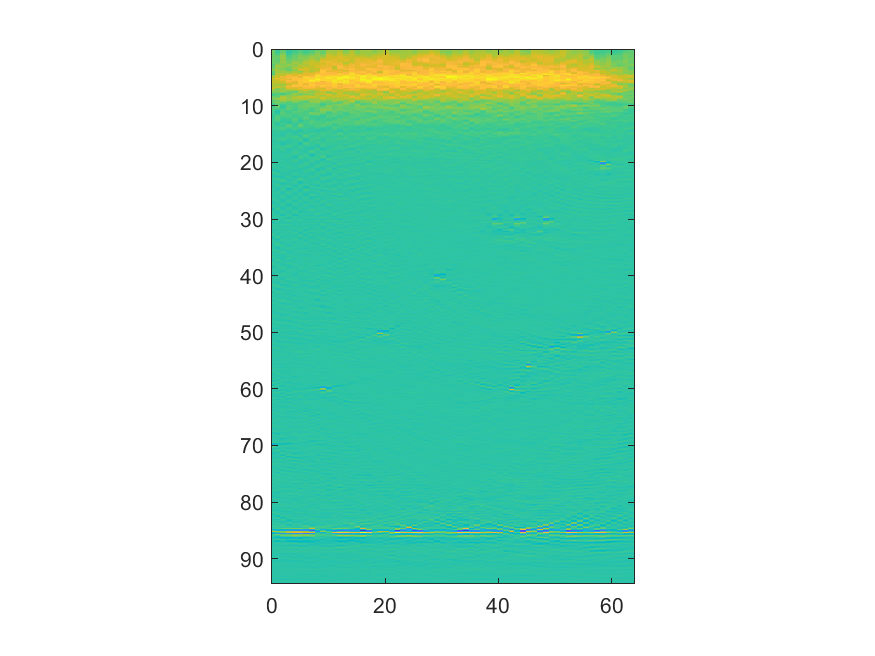
\includegraphics[width=1.1\textwidth]{O_1}
                \end{minipage}}
                \hfill
                \subfloat[$N_x = 2048$]{
                    \begin{minipage}[c][1\width]{
                        0.5\textwidth}
                        \centering
                        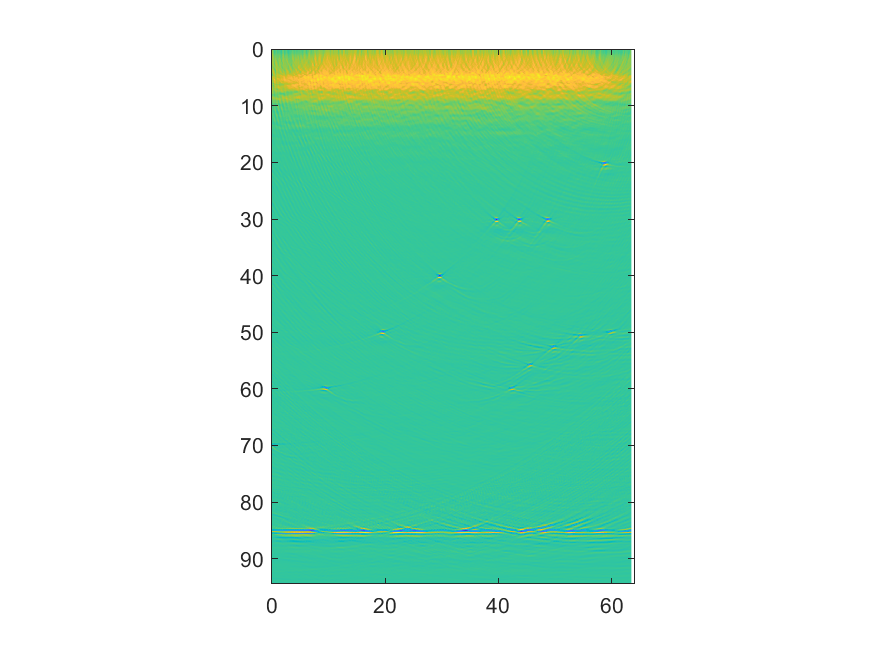
\includegraphics[width=1.2\textwidth]{O_6}
                \end{minipage}}
                \caption{}
            \end{figure}

    On observe que les trous sont bien plus faciles à distinguer sur la
    figure correspondant à $N_x = 2048$ que sur la première, correspondant
    à $N_x = 64$.

    Les temps de calcul associés sont respectivement :
    0.27s, 0.43s, 0.86s, 1.75s, 3.38s et 6.74s.

    Ainsi, on observe que la complexité est linéaire en $N_x$.
        }
\end{itemize}

\section{Post-traitement de l'image}

Affichons une image $O$ obtenue après post-traitement :

            \begin{figure}[H]
                \caption{Image $O$ après post-traitement}
                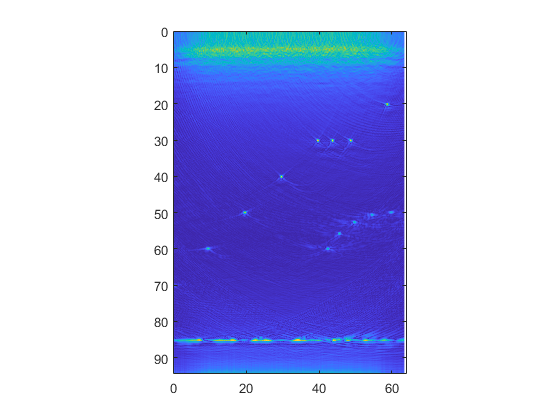
\includegraphics[width=0.5\textwidth]{O_hilbert}
                \centering
            \end{figure}

On observe alors que le post-traitement a permis de gagner en
lisibilité en jouant sur les couleurs.
En effet, les trous de la plaque ressortent beaucoup plus du fond.

\section{Accéleration avec une fonction MEX}

Le contenu du fichier \texttt{MEX\_SAFT.c} est disponible en annexe.

\section{Comparaisaon de deux mises en oeuvre}

\begin{itemize}
    \item{Commençons par afficher une des images obtenues pour chaque version :

            \begin{figure}[H]
                \caption{Deux images $O$}
                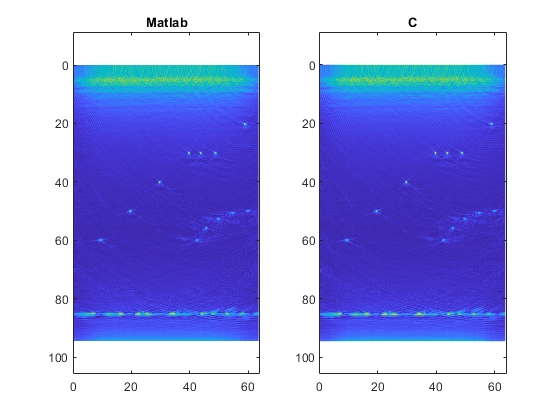
\includegraphics[width=0.7\textwidth]{cmp}
                \centering
            \end{figure}

            Ces images semblent être identiques, c'est le cas pour toutes les valeurs de $N_x$.
        }
    \item{Affichons le temps de calcul des deux versions :

            \begin{figure}[H]
                \caption{Temps de calcul}
                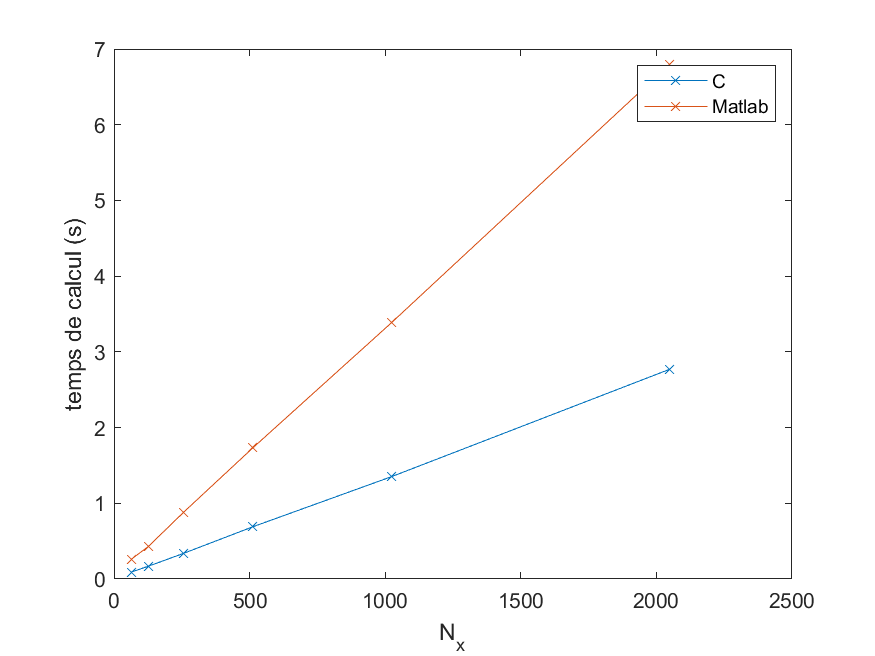
\includegraphics[width=0.5\textwidth]{temps}
                \centering
            \end{figure}

            La complexité est évidemment inchangée entre les les deux versions mais la version en MEX
            est environ 60\% plus rapide que la version Matlab. Cette différence est entièrement
            due aux différences entre les deux langages. Le langage C, étant bas niveau, est
            connu pour sa rapidité.
        }
    \item{Affichons la ligne $z = 30$

            \begin{figure}[H]
                \caption{Ligne $z = 30$}
                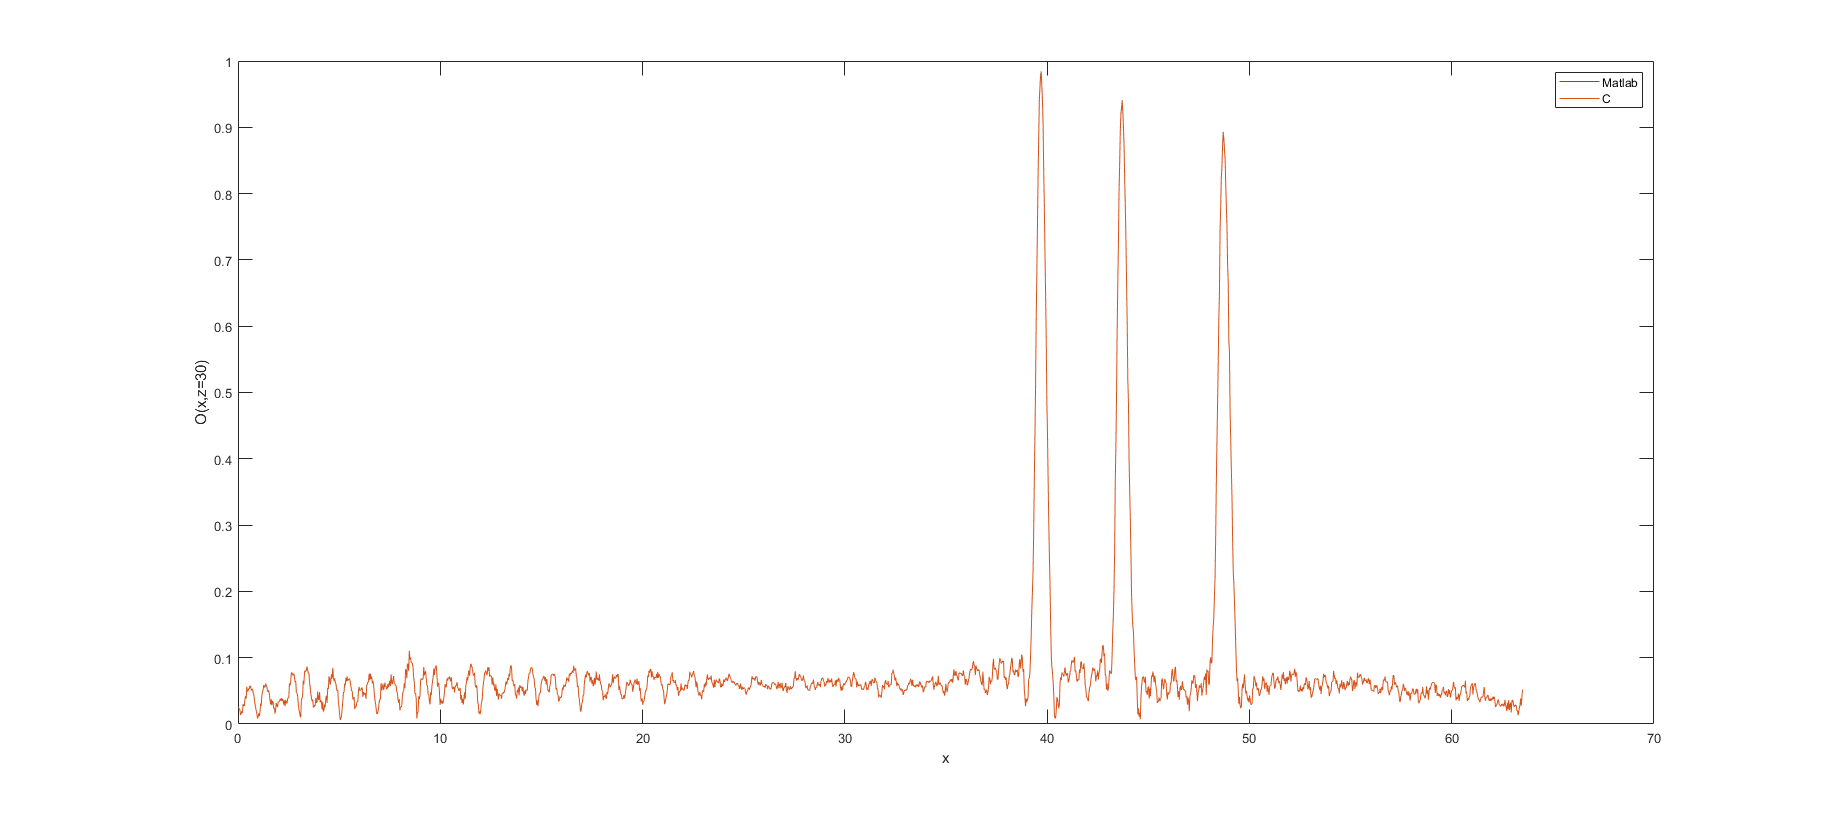
\includegraphics[width=0.7\textwidth]{ligne}
                \centering
            \end{figure}

            Les trous dans la direction $x$ sont espacés d'environ 5 cm.

            Affichons enfin la différence :

            \begin{figure}[H]
                \caption{Différence entre les deux signaux}
                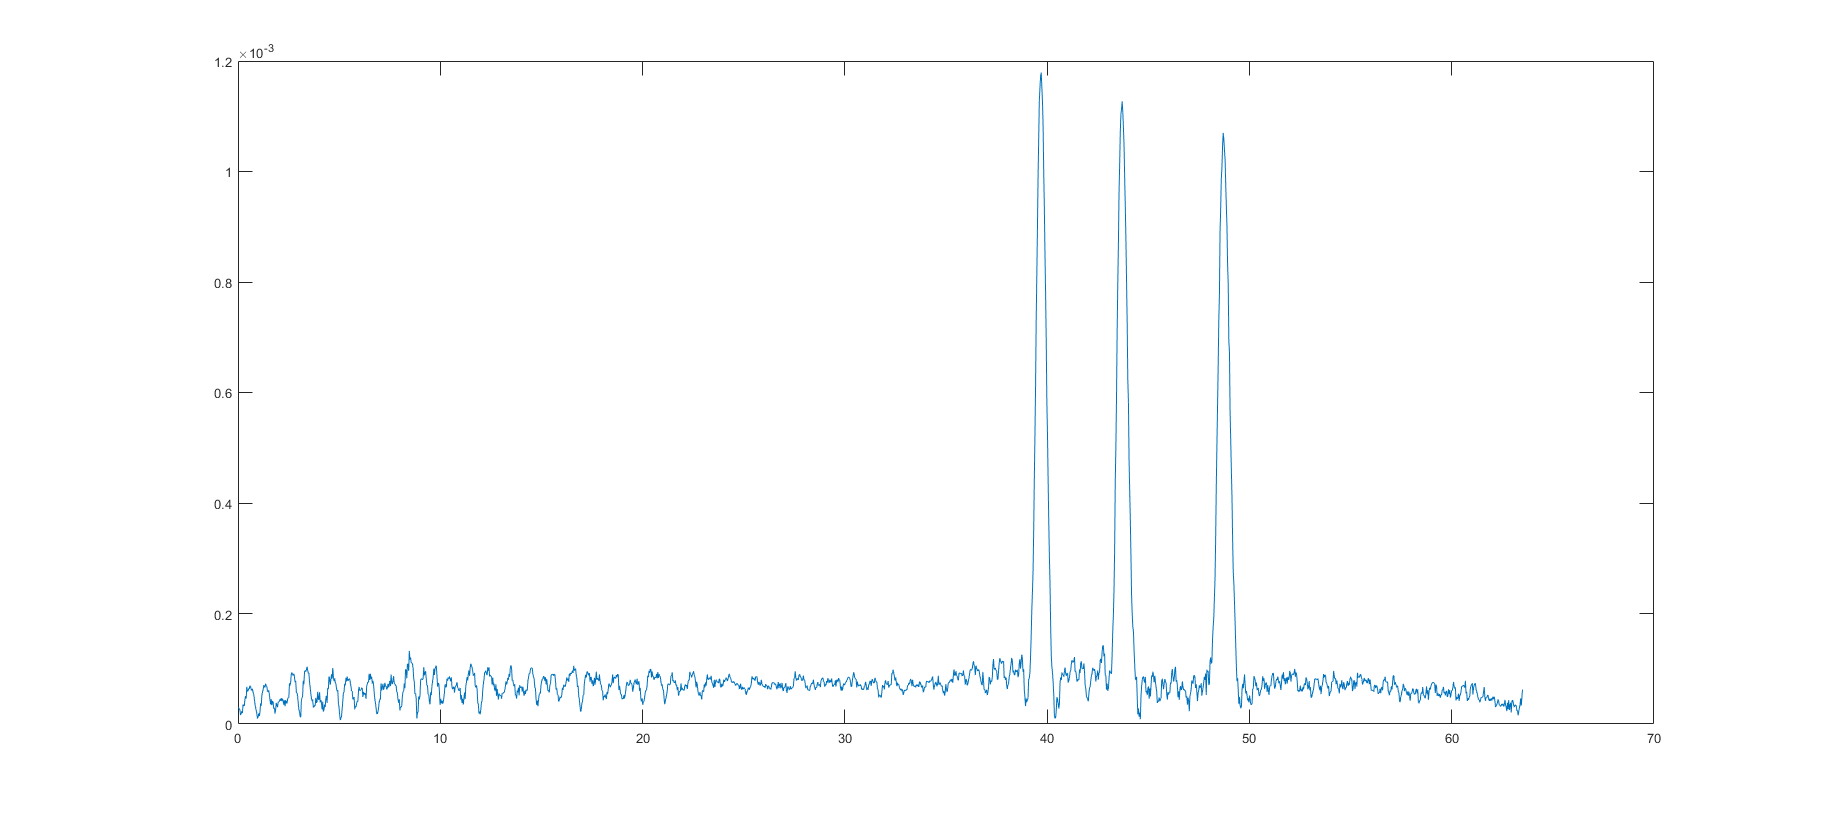
\includegraphics[width=0.7\textwidth]{diff}
                \centering
            \end{figure}

            Cette différence n'est pas nulle. Il y alors une différence entre les deux signaux.
            En effet, en les observant de plus près, on note la présence d'un léger retard entre
            ces signaux.
        }
\end{itemize}

\section*{Conclusion}

Ainsi, lors de ce TP nous avons pu implémenter une méthode d'imagerie temporelle afin d'observer les
petits trous de la plaque. Nous avons pu comparer les performances de la procédure entre une version
matlab et MEX. On a alors conclu que la version MEX était environ 60\% plus rapide que son équivalent
Matlab.

\pagebreak

\begin{appendices}
    \section{\texttt{Main.m}}

    \lstinputlisting[language=Matlab]{../main.m}

    \section{\texttt{MEX\_SAFT.c}}

    \lstinputlisting[language=C]{../MEX_SAFT.c}
\end{appendices}

\end{document}
